\section{Architecture}
\label{sec:architecture}

\subsection{One object per frame}

Everything a stage can read or write for the frame in front of it lives on a
single object, \texttt{Ctx}, which the runner creates per frame and discards at
the end of it. It carries the working image, the untouched source frame, the
frame index, and four output channels that are kept apart on purpose:

\begin{description}
  \item[\texttt{store}] a side channel within one frame: an artifact one stage
    produces and a later stage consumes, such as the binary mask
    \texttt{static\_mask} publishes and \texttt{apply\_mask} reads. It is thrown
    away when the frame ends. State that has to survive between frames belongs on
    the stage instance instead, and the distinction is enforced by the fact that
    nothing carries \texttt{store} forward.
  \item[\texttt{taps}] a snapshot of the working image taken after each
    \emph{named} stage, so a sink can write a mid-chain frame instead of only the
    final one. Taps are filled by the runner, never by a stage. Keeping them out
    of \texttt{store} is what stops a stage named \texttt{mask} from shadowing the
    unrelated \texttt{store["mask"]} artifact --- a collision that would be
    invisible until it produced a wrong picture.
  \item[\texttt{metrics}] the per-frame scalars a stage measured:
    \texttt{edge\_px}, \texttt{contours}, \texttt{motion\_speed},
    \texttt{lbp\_entropy}. One dictionary per frame, and what the JSON sink
    writes.
  \item[\texttt{rows}] per-object detail --- one list of flat records per kind.
    This is separate from \texttt{metrics} because a single frame's
    \texttt{contours = 400} metric can have four hundred records behind it, and
    the CSV and crop sinks want those records, not the count.
\end{description}

A stage's contract is one method, \texttt{apply(ctx)}, and one rule: rebind
\texttt{ctx.image} to a new array, never modify the array in place. The rule
exists because \texttt{image} and \texttt{source} alias the same buffer when a
frame enters the chain and no defensive copy is taken --- at these frame rates a
per-frame copy is pure waste. A sink's contract is \texttt{write(ctx)}, returning
\texttt{False} to stop the run, which is how a preview window's quit key ends a
batch.

\subsection{Almost nothing has state}

Of the \NumStages{} stages, the ones that remember anything between frames are
the motion models and the background models, and they remember it on themselves.
There is exactly one state machine in the codebase --- the fixed background model
is either still accumulating its first $N$ frames or has fitted its mean and is
subtracting it --- and everything else is either a pure function of the current
frame or a running accumulation. That is a small fact with a large consequence:
it is why the analysis in §\ref{sec:optimizer} can rearrange a chain and know
what it is allowed to conclude, and why a chain's behaviour is a property of the
config rather than of the order somebody happened to click things.

\begin{figure}[t]
  \centering
  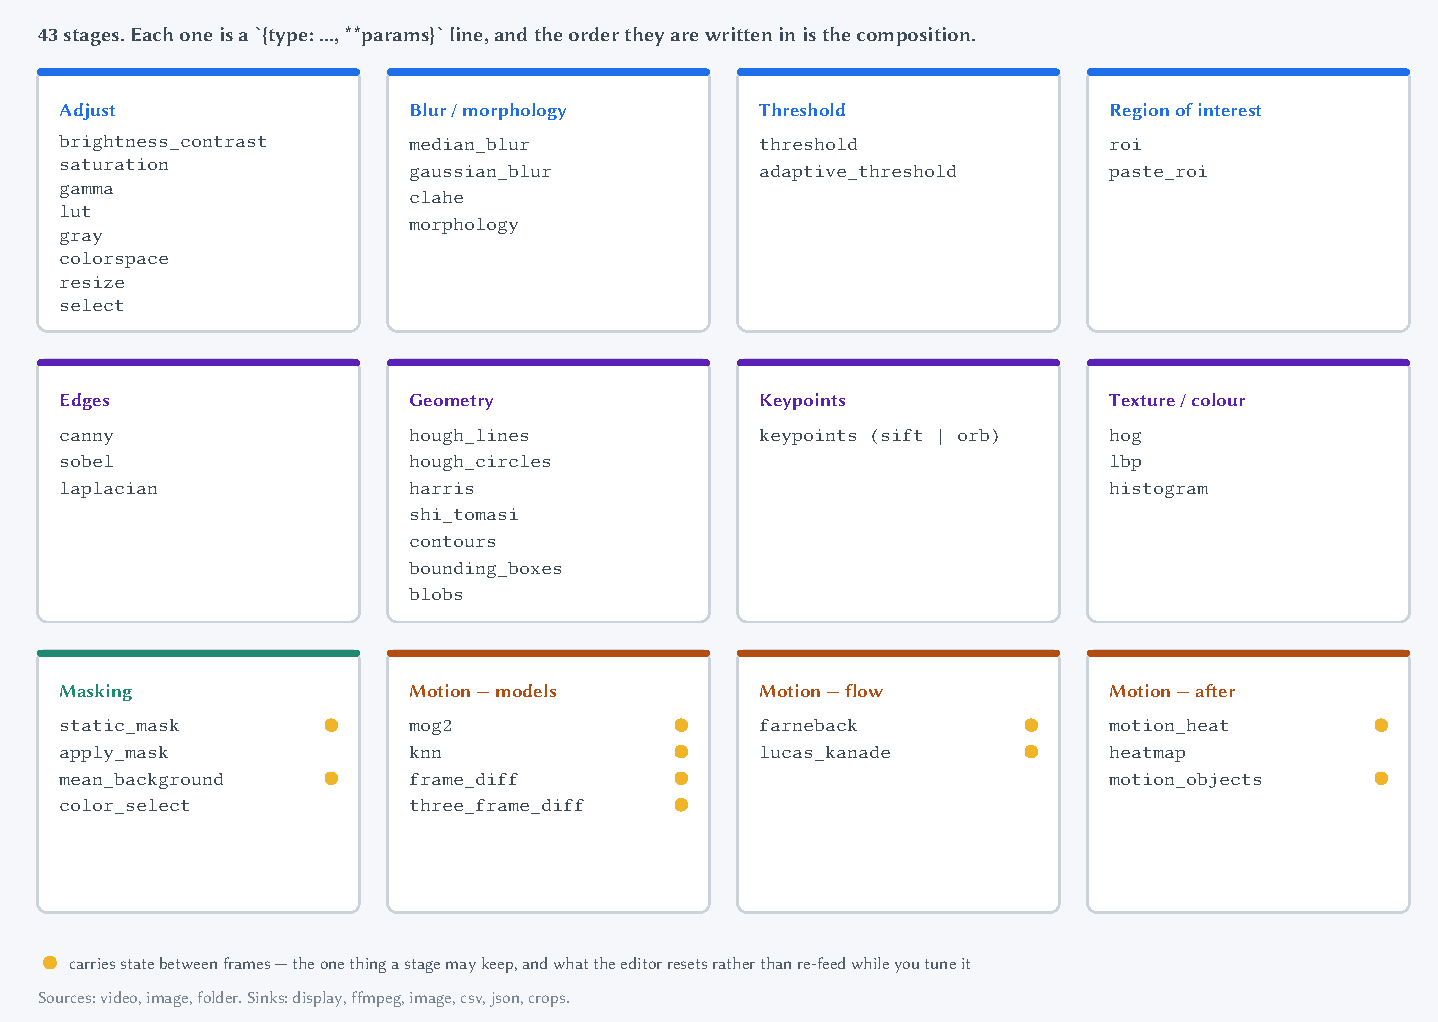
\includegraphics[width=\textwidth]{figures/stage-families.pdf}
  \caption{The \NumStages{} registered stages, grouped as the editor's palette
    groups them for browsing. The source tree divides them differently, into the
    \NumFamilies{} modules the appendix is organised by: \FamilyList{}.}
  \label{fig:families}
\end{figure}

\subsection{Where the operators come from}

None of the \NumStages{} operators is novel, and that is the point: each one is a
published method with three decades of use behind it, wrapped so that a config
can name it. The structure family implements Canny's edge detector
\cite{canny1986}, the Harris--Stephens corner response \cite{harris1988} and the
Shi--Tomasi selection criterion derived from it \cite{shi1994}, border-following
contour extraction \cite{suzuki1985}, and the progressive probabilistic Hough
transform for line segments \cite{matas2000}. The motion family covers sparse
Lucas--Kanade flow \cite{lucas1981}, dense flow by polynomial expansion
\cite{farneback2003}, and the two adaptive background subtractors --- the
improved Gaussian mixture model \cite{zivkovic2004} and its per-pixel density
estimation successor \cite{zivkovic2006}. The texture family provides histograms
of oriented gradients \cite{dalal2005} and multiresolution local binary patterns
\cite{ojala2002}; contrast-limited adaptive histogram equalisation
\cite{zuiderveld1994} sits in preprocessing. The implementations are OpenCV's
\cite{bradski2000} and scikit-image's \cite{vanderwalt2014} over NumPy arrays
\cite{harris2020numpy}; what this project contributes is the composition, not the
operators.

The two exceptions are worth naming because they are the only stages with no
published counterpart: the fixed region mask and the mean-of-$N$ background were
written for this project's own footage, and they are the two the predecessor
script already had.

\subsection{Why ordering has to be the composition}

\begin{figure}[t]
  \centering
  \begin{subfigure}[t]{0.48\textwidth}
    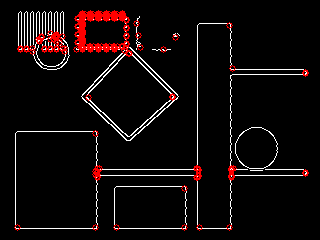
\includegraphics[width=\textwidth]{figures/ordering-edges-first.png}
    \caption{\texttt{canny} then \texttt{harris}: corners drawn onto the edge map.}
  \end{subfigure}\hfill
  \begin{subfigure}[t]{0.48\textwidth}
    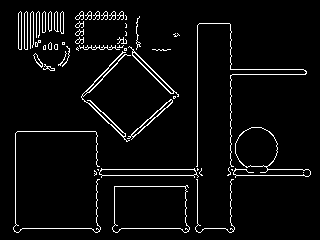
\includegraphics[width=\textwidth]{figures/ordering-corners-first.png}
    \caption{\texttt{harris} then \texttt{canny}: the corner markers are reduced
      to outlines, and an extra \texttt{gray} is needed to get there.}
  \end{subfigure}
  \caption{Ordering is the composition. The same two operators in opposite order
    are not two settings of one pipeline; they are two different pipelines.}
  \label{fig:ordering}
\end{figure}

Figure~\ref{fig:ordering} is the argument in one picture. Both panels run
\texttt{canny} and \texttt{harris} on the same frame with the same parameters.
On the left, edges are found first and the corner detector draws onto the edge
map, which is how you check that a corner detector is looking at the structure
you think it is. On the right, corners are drawn first and the edge detector then
runs over the markers and reduces them to outlines --- and because the marker
overlay is in colour, the reversed order also needs a \texttt{gray} stage
inserted to get there at all.

No flag distinguishes those two pipelines. A system that tried to express this
with options would need a \texttt{draw\_over\_edges} boolean, and then another
one for the next pair, and each would be a branch taken at runtime that somebody
has to read the source to understand. Making position the only composition
operator means the file shows what happens in the order it happens, and the cost
is paid in exactly one place: an operator that needs an image other than the one
in front of it has to say so. Several do --- \texttt{draw\_on: source} paints on
the original frame, \texttt{input: edges} reaches back to a named tap,
\texttt{mask: mask} reads a published artifact --- and those parameters are
visible in the config rather than implied by it.
